\subsection{Trigger di Schmitt non-invertente}

\begin{wrapfigure}[16]{r}{0.50\textwidth}
  \begin{center}
    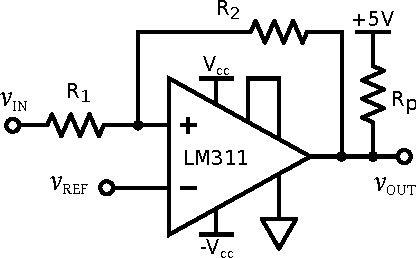
\includegraphics[width=0.320\textwidth]{../E04/latex/c_schmitt.pdf}
  \end{center}
  \caption{Schema del trigger di Schmitt. Le resistenze $R_1$ e $R_2$ sono state variate, mentre $R_p=(9.98 \pm 0.01)$ \si{\kilo\ohm}, come consigliato sul datasheet.}
  \label{cir4:schmitt}
\end{wrapfigure}

Quando nel segnale è presente un rumore è possibile che il valore di tensione restituito dal comparatore cambi più volte da $0$ a $V_{C}$.
Infatti, l'ampiezza in tensione del rumore può essere tale da passare sopra e sotto la tensione di soglia, invertendo la $V_{out}$ più volte, in accordo con (\ref{eq4:comparatore}).

Per ovviare a questo problema si sfrutta la retroazione positiva dell'amplificatore operazionale per riportare parte della $V_{out}$ sull'ingresso non invertente: ciò permette di creare un offset positivo sulla tensione all'ingresso non invertente quando $V_{in}>0$ e viceversa.
Quindi, durante il confronto del segnale con la tensione di riferimento, il segnale in entrata risulterà aumentato o diminuito di una certa quantità a seconda di $V_{out}$.

Valutiamo queste tensioni di soglia nel trigger di Schmitt non invertente (grafico in Figura \ref{cir4:schmitt}).
Per fare ciò cerchiamo la dipendenza di $V_{in}$ da $V_{out}$ e da $V^+$ (tensione all'ingresso non invertente). Utilizzando la legge di Kirchhoff sul nodo dell'ingresso non invertente
$$\frac{V_{in}-V^+}{R_1} + \frac{V_{out}-V^+}{R_2} = 0$$
da cui otteniamo
\begin{equation}
V_{in} = V^+ \frac{R_1+R_2}{R_2} - V_{out} \frac{R_1}{R_2}
\label{eq4:v_in_parte2}
\end{equation}
Dunque otteniamo i valori di soglia (che sono valori di $V_{in}$) ponendo la tensione $V^+=V^-=V_{ref}=0$, cioè il punto di tensione di inversione del comportamento del LM311 a collettore comune, e considerando i due valori possibili di $V_{out}$ dati dalla (\ref{eq4:comparatore}), cioè $V_{out}^{inf}=0$ e $V_{out}^{sup}=V_{C}=5$\si{\volt}:
$$V_{soglia}^{sup} = - V_{out}^{inf} \frac{R_1}{R_2} = 0 \qquad V_{soglia}^{inf} = - V_{out}^{sup} \frac{R_1}{R_2} = - (0.46 \pm 0.01) \si{\volt}$$
da cui è possibile definire la tensione di \textit{isteresi} (cioè la tensione massima in cui un segnale può oscillare attorno alla tensione di riferimento prima di ribaltare l'output del LM311)
$$V_{isteresi} = |\Delta V| = |V_{soglia}^{sup} - V_{soglia}^{inf}| = V_{out}^{sup} \frac{R_1}{R_2} = (0.46 \pm 0.01) \si{\volt}$$

I punti così calcolati sono visibili nel grafico di isteresi in Figura \ref{gr4:isteresi}.

Notiamo però che vi sono alcune incongruenze rispetto al grafico ideale di isteresi: le rette $V_{in}=V_{soglia}$ (per entrambe le soglie) in realtà non sono perpendicolari alle ascisse, e abbiamo ipotizzato che tale comportamento sia imputabile all'entrata dell'opamp in regione lineare, uscendo dalla saturazione.
Inoltre la tensione di uscita massima non è $5$ \si{\volt} perché, a differenza del comparatore in Figura \ref{cir4:comparatore}, la corrente quando Q è interdetto può passare attraverso il circuito di retroazione, provocando una caduta di potenziale sulla resistenza $R$.
Tale corrente dipende inoltre dalla tensione in entrata, dunque è spiegata la pendenza della retta $V_{out}^{sup}$.

Abbiamo infine provato ad inserire un offset all'ingresso invertente: ciò ha portato, come ci aspettavamo dalla relazione (\ref{eq4:v_in_parte2}) (si ricorda che $V^+=V_{ref}$), ad una traslazione del grafico in Figura \ref{gr4:isteresi} di un valore dato dall'offset impostato. Infine, durante l'esperienza, abbiamo anche variato $R_1$ per valutare diverse tensioni di isteresi.

\begin{figure}[ht]
 \centering
   {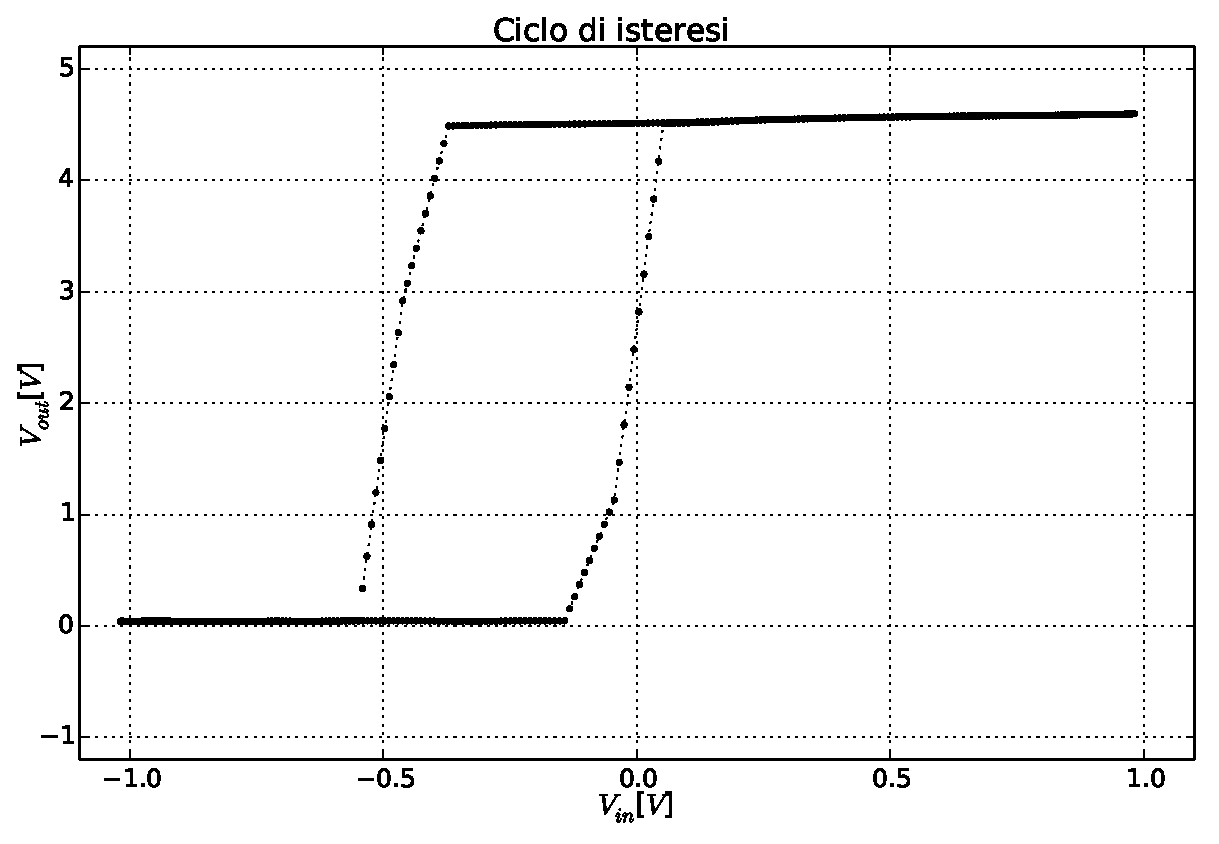
\includegraphics[width=14.5cm]{../E04/latex/XY.pdf}}
 \caption{Grafico dell'isteresi. Per questi dati le resistenze utilizzate sono $R_1=\SI{9.98(1)}{\kohm}$ e $R_2=\SI{99.6(1)}{\kohm}$. Le varie differenze rispetto al grafico ideale sono spiegate nel paragrafo.}
 \label{gr4:isteresi}
\end{figure}